\documentclass[a4paper,10pt]{article}
\usepackage[utf8]{inputenc}
\usepackage[T1]{fontenc}
\usepackage{graphicx}
\usepackage[top=2cm,bottom=2cm]{geometry}
\usepackage[labelformat=empty]{caption}
\usepackage{fancyhdr}
\pagestyle{fancy}
\usepackage{anslistings}

\begin{document}
    \title{Envariabelanalys \\ Inlämningsuppgift 2}
    \date{\today}
    \author{Jakob Larsson}
    \maketitle
    \rhead{Jakob Larsson TKDES-1. \today}

    \section*{2.1}

    \begin{samepage}
        \inputmatlabnt{backwardEulerSyst.m}
    \end{samepage}
    \begin{samepage}
        \inputmatlabnt{fixedpointVec.m}
    \end{samepage}
    \begin{samepage}
        \inputmatlabnt{mpEulSyst.m}
    \end{samepage}

    \section*{2.2}
    \begin{samepage}
        \inputmatlabnt{svang.m}
    \end{samepage}
    \begin{samepage}
        \inputmatlabnt{svangTest.m}
    \end{samepage}

    \begin{figure}
        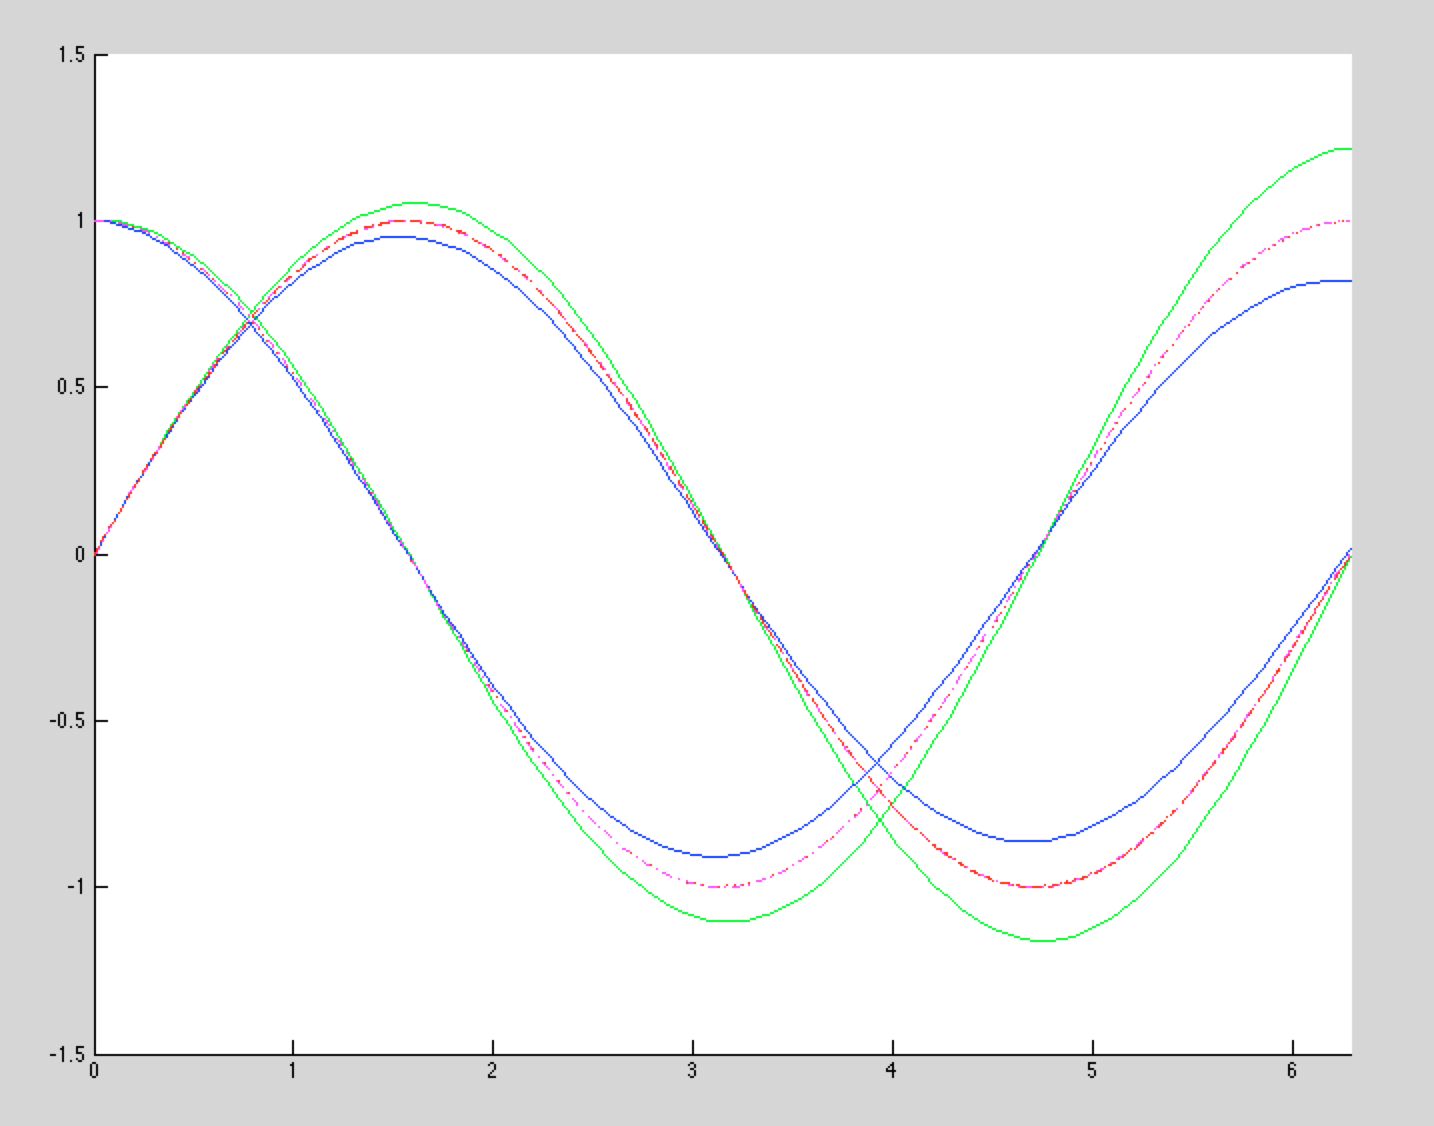
\includegraphics[width=\textwidth]{svang.png}
        \caption{Grön är framåt, blå är bakåt.
            Mittpunkt, ode45 och den analytiska lösningen ligger alla i samma
            linje så de är svåra att urskillja.}
    \end{figure}

    \section*{2.3}
    Mina framåt och bakåtlösare fick en singulärpunkt med de angivna begynnelsevärdena och kan därför inte användas. Därför är bara mittpunktslösaren redovisad i grafen. Större värden på N ger en bättre approximation och det tar längre tid innan mina lösare löper "amok".

    Om man tredublar den lilla planetens hastighet snurrar den snabbare runt den stora planeten. Om man tiodubblar sliter den sig loss från sin bana direkt.
    \begin{samepage}
        \inputmatlabnt{celest2.m}
    \end{samepage}
    \begin{samepage}
        \inputmatlabnt{celest2Test.m}
    \end{samepage}

    \begin{figure}
        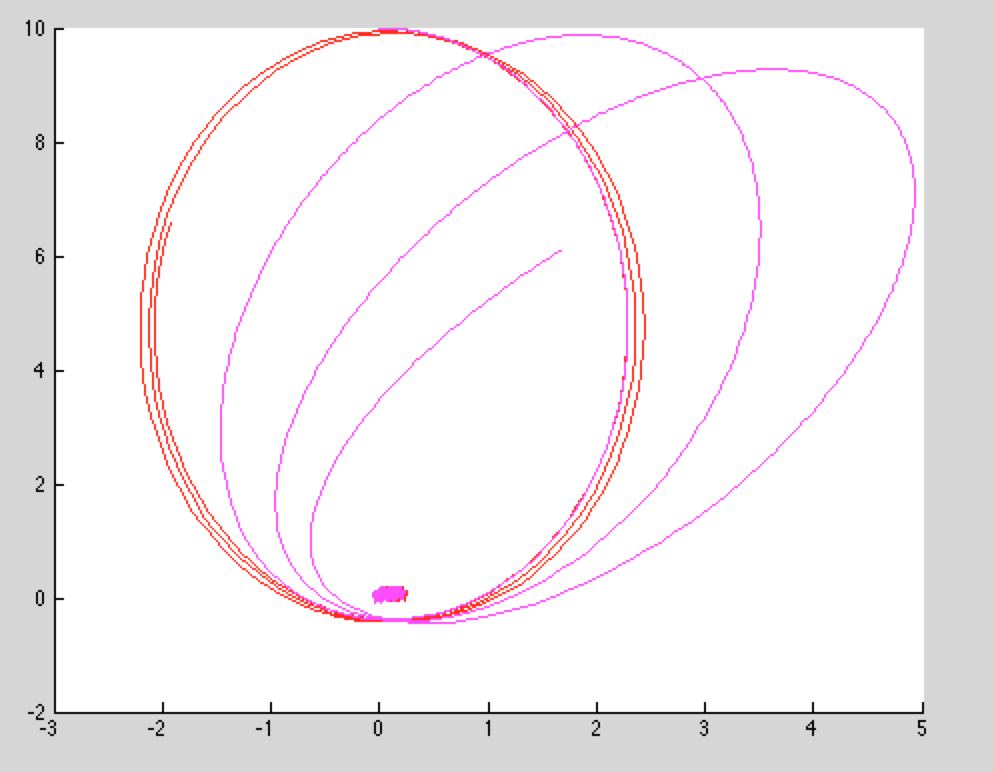
\includegraphics[width=\textwidth]{celest2.png}
        \caption{Två planeter i planet.}
    \end{figure}

    \section*{2.4}
    Jag har inte bifogat för ledningen av $(6)$ här. Jag har inte orkat skriva rent den tyvärr och jag tycker att det är en väldigt trivial uppgift.
    Om man ändrar månens begynnelsevärden mer än ytterst lite slutar månen att gå runt jorden.
    \begin{samepage}
        \inputmatlabnt{celest3.m}
    \end{samepage}
    \begin{samepage}
        \inputmatlabnt{celest3Test.m}
    \end{samepage}

    \begin{figure}
        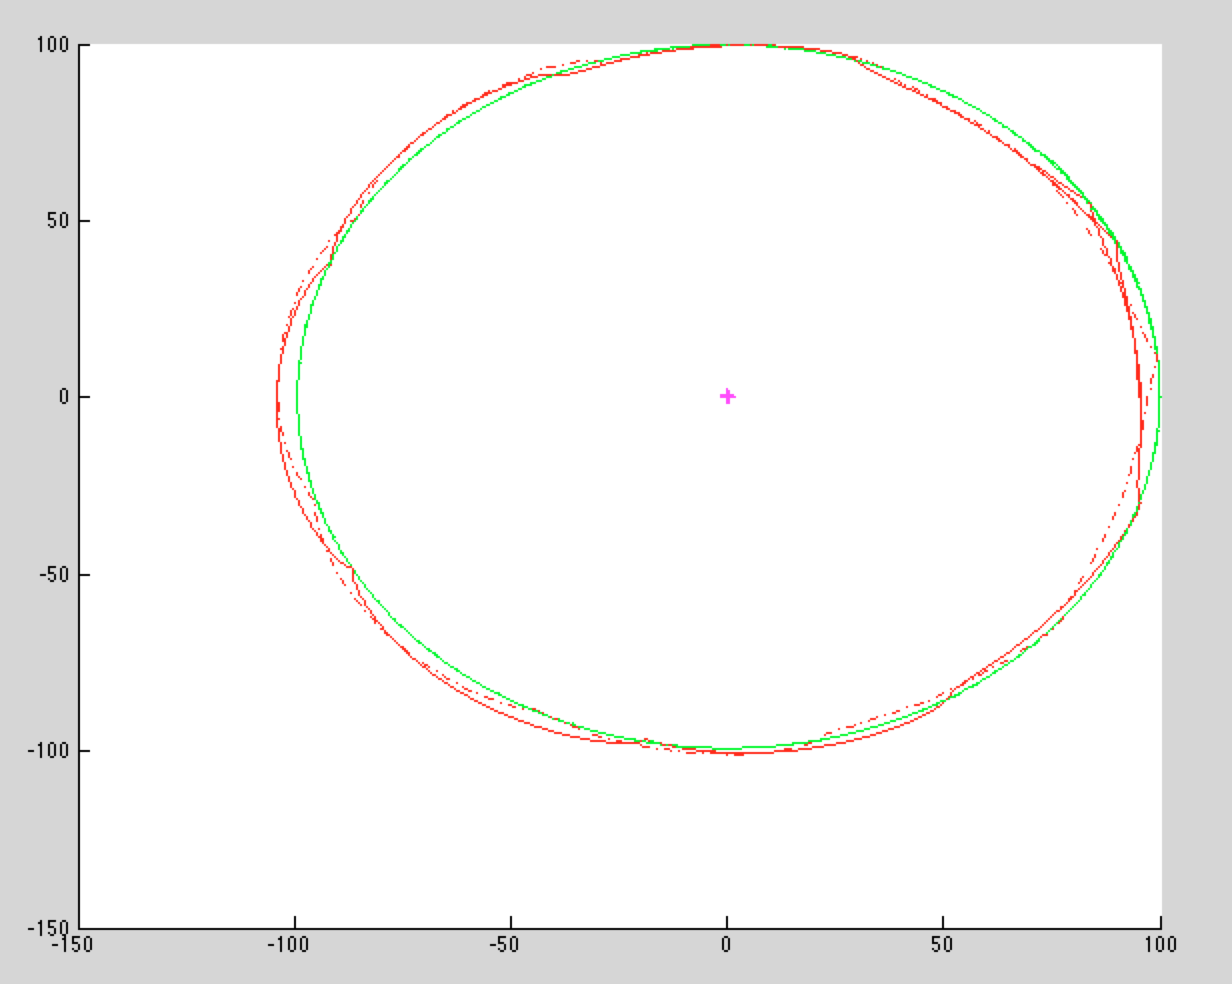
\includegraphics[width=\textwidth]{celest3.png}
        \caption{Tre planeter i två dimensioner. Den streckade linjen är ode45.}
    \end{figure}

    \section*{2.5}
    För ode15s tog det 0.0891s och för ode45 93.065s.
    Tidsvektorn för ode15s och ode45 har 227 respektive 2376197 element.

    ode45 använder väldigt många partitioner för att aproximera lösningsfunktionen
    bra. Därmed tar det också lång tid.
    ode15s är så smart att den tar små steg där det behövs och stora där funktionen är mer stabil. För vissa funktioner betyder det en lika bra approximation på mindre tid.
    \begin{figure}
        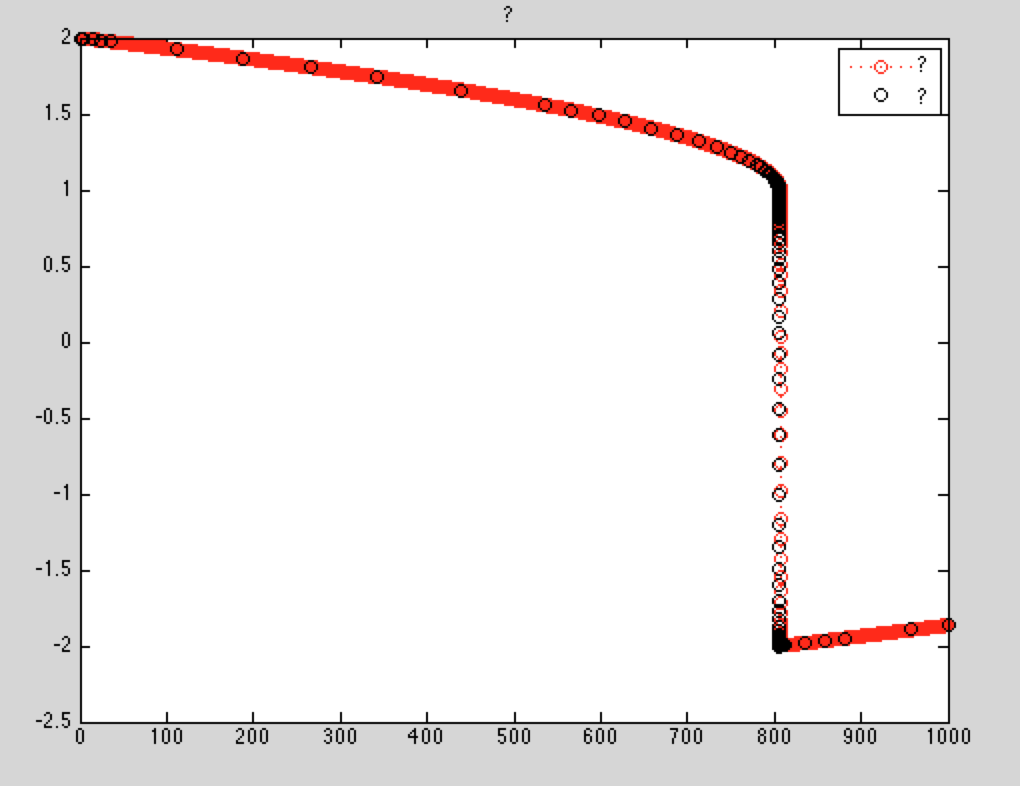
\includegraphics[width=\textwidth]{vdpool1000.png}
        \caption{Lösningsplott av vdpool.m på [0 1000].}
    \end{figure}

    \section*{2.6}
    \begin{samepage}
        \inputmatlabnt{celest33d.m}
    \end{samepage}
    \begin{samepage}
        \inputmatlabnt{celest33dTest.m}
    \end{samepage}

    \begin{figure}
        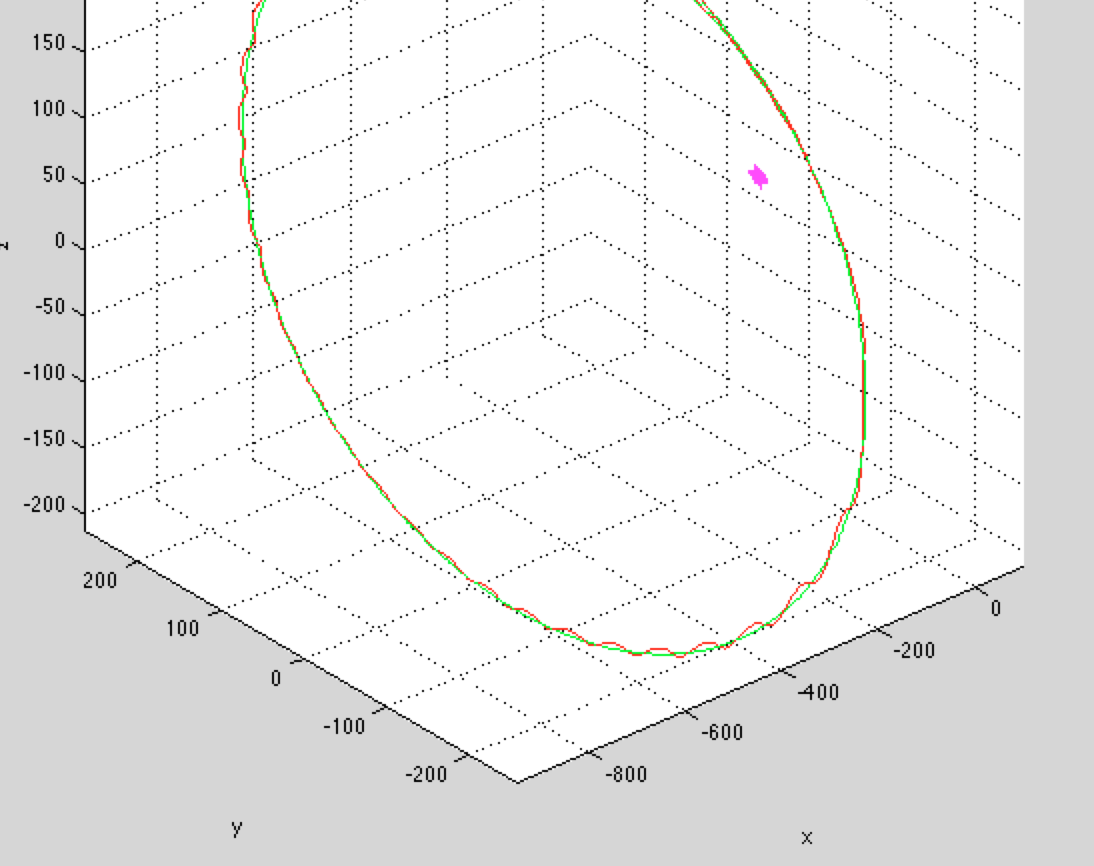
\includegraphics[width=\textwidth]{celest33d.png}
        \caption{Tre planeter i 3 dimensioner.}
    \end{figure}

    \section*{2.7}
    Ungefär 24 timmar.

\end{document}
